\chapter{大观园试才题对额\quad 荣国府归省庆元宵}
\ji{此回宜分二回方妥\foot{按:己、庚本第十七至十八回未分回,直接题为“第十七回至十八回”。
为兼顾戚、蒙本的回前回后批,本校本仍予分回。
}。
\hang
宝玉系诸艳之冠,故大观园对额必得玉兄题跋,且暂题灯匾联上,
\zhu{
灯匾联:匾额和对联的腔体内部设置灯烛,使得能在夜里看清题写之字。
第十八回元妃夜览大观园方能看清所题之字。
}
再请赐题,此千妥万当之章法。
}\par
诗曰:\par
豪华虽足羡,离别却难堪。
博得虚名在,谁人识苦甘?\ji{好诗,全是讽刺。
近之谚云:“又要马儿好,又要马儿不吃草。
”真骂尽无厌贪痴之辈。
}\par
\hop
话说秦钟既死,宝玉痛哭不已,李贵等好容易劝解半日方住,归时犹是凄恻哀痛。
贾母帮了几十两银子,外又另备奠仪,宝玉去吊纸。
\zhu{吊纸:这里指在死者灵前烧纸吊祭。
}七日后便送殡掩埋了,别无述记。
只有宝玉日日思慕感悼,然亦无可如何了。
\ji{每于此等文后便用此语作结,是板定大章法,
\zhu{板定:一定,必定。}
亦是此书大旨。
}\par
又不知历几何时,\ji{年表如此写,亦妙!}\geng{惯用此等章法。
}这日贾珍等来回贾政:“园内工程俱已告竣,大老爷已瞧过了,只等老爷瞧了,或有不妥之处,再行改造,好题匾额对联的。
”贾政听了,沉思一回,说道:“这匾额对联倒是一件难事。
论理该请贵妃赐题才是,然贵妃若不亲睹其景,大约亦必不肯妄拟;若直待贵妃游幸过再请题,\zhu{游幸:旧称帝王、后妃的行动所至为“幸”,如到某地称“幸某地”,游赏称“游幸”。
}偌大景致,\zhu{
偌:音“若”,如此,这样。
偌大:这么大。
}
若干亭榭,无字标题,也觉寥落无趣,任有花柳山水,也断不能生色。
”众清客在旁笑答道:“老世翁所见极是。
如今我们有个愚见:各处匾额对联断不可少,亦断不可定名。
如今且按其景致,或两字、三字、四字,虚合其意,拟了出来,暂且做出灯匾联悬了。
待贵妃游幸时,再请定名,岂不两全?”贾政等听了,都道:“所见不差。
我们今日且看看去,只管题了,若妥当便用;不妥时,然后将雨村请来,令他再拟。
”\ji{点雨村,照应前文。
}众人笑道:“老爷今日一拟定佳,何必又待雨村。
”贾政笑道:“你们不知,我自幼于花鸟山水题咏上就平平;\geng{是纱帽头口气。
\zhu{纱帽:古代文官所戴的帽子。后用作官职的代称。}
}如今上了年纪,且案牍劳烦,于这怡情悦性文章上更生疏了,纵拟了出来,不免迂腐古板,反不能使花柳园亭生色,似不妥协,反没意思。
”\geng{政老情字如此写。
壬午季春。
畸笏。
}众清客笑道:“这也无妨。
我们大家看了公拟,各举其长,优则存之,劣则删之,未为不可。
”贾政道:“此论极是。
且喜今日天气和暖,大家去逛逛\ji{音光,字去声,出《谐声字笺》。
}。
”说着起身,引众人前往。
\par
贾珍先去园中知会众人。
可巧近日宝玉因思念秦钟,忧戚不尽,贾母常命人带他到园中来戏耍。
\geng{现成榫楔,
\zhu{
榫:音“损”,制做木器时,以凹凸相入接合两件材料,其中凸的部分即称为「榫」。
楔[xiē]:上平厚、下尖扁的木块。塞在榫头缝隙中,使之固定。
}
一丝不费力。
若特唤出宝玉来,则成何文字?}此时亦才进去,忽见贾珍走来,向他笑道:“你还不出去,老爷就来了。
”宝玉听了,带着奶娘小厮们,一溜烟就出园来。
\geng{不肖子弟来看形容。
余初看之,不觉怒焉,盖谓作者形容余幼年往事,因思彼亦自写其照,何独余哉?信笔书之,供诸大众同一发笑。
}方转过弯,顶头贾政引众客来了,躲之不及,只得一边站了。
贾政近日因闻得塾掌称赞宝玉专能对对联,
\zhu{
塾掌:塾:私塾。
旧时民间办的学校。
私塾的主管者,叫“塾掌”。
}
虽不喜读书,偏倒有些歪才情似的,\meng{如此顺笔写来,然却是宝玉正传。
}今日偶然撞见这机会,便命他跟来。
\ji{如此偶然方妙,若特特唤来题额,真不成文矣。
}宝玉只得随往,尚不知何意。
\par
贾政刚至园门前,只见贾珍带领许多执事人来,一旁侍立。
贾政道:“你且把园门都关上,我们先瞧了外面再进去。
”\geng{是行家看法。
}贾珍听说,命人将门关了。
贾政先秉正看门。
\zhu{秉正:这里是摆正了姿势、选正了位置的意思。
秉:执;把握。
}只见正门五间,上面桶瓦泥鳅脊;\zhu{桶瓦泥鳅脊:指“卷棚顶”,图见页脚\foot{\footPic{卷棚顶}{juanpeng.jpg}{1.0}}。
卷棚:建筑术语,指屋面两坡的连接处不用正脊压盖,而使用桶瓦(半圆筒形的瓦),这样两坡相交处成弧形的曲面,状如泥鳅,所以称“泥鳅脊”。
}那门栏窗槅,
\zhu{窗槅:亦称“窗隔”、“窗格”。窗上的格子,古时在上面糊纸或纱以挡风,亦指窗扇。}
皆是细雕新鲜花样,并无朱粉涂饰;一色水磨群墙,\zhu{水磨群墙:窗台和腰线石以下的墙体称群墙,用磨砖对缝作法砌筑。
磨砖对缝:古代建筑中的一种高级建筑工艺,即将毛砖砍磨成边直角正的长方形等,砌筑成墙时,以江米米汤和白灰浆为粘合剂,使砖的缝隙弥合,最终使得整个墙面光滑平整,严丝合缝\foot{
\footPic{磨砖对缝砌筑的墙面}{mozhuan.jpg}{0.6}
}。
水磨:为了使砖面能够磨得足够细,一般还要先把砖浸到水里,这也就是后世所谓“水磨方砖”说法的由来。
另一种说法是墙砌好之后,还需用细磨石沾水磨光,因此叫做“水磨群墙”。
}
\ji{门雅,墙雅,不落俗套。
}下面白石台矶,凿成西番草花样。
\zhu{西番草花样:一种连续不断的西番草图案。
西番草即西番莲,常绿缠绕植物,夏季开花,也叫缠枝莲。
}左右一望,皆雪白粉墙,\zhu{粉墙:涂刷成白色的墙。
粉墙黛瓦指雪白的墙壁,青黑的瓦,用来描写房屋。
}下面虎皮石,
\zhu{
虎皮石:有斑纹的墙。以大小不整、各种形状的石块砌成墙脚,并以灰勾出轮廓,因似虎皮斑纹,故称。
清·李光庭《乡言解颐》卷二:“北地以余所见,则蓟州、三河墙屋,多用不方不圆者甃砌,合缝以灰钩之,谓之虎皮石,既坚且耐观。”
}
随势砌去,果然不落富丽俗套,自是欢喜。
遂命开门,只见迎门一带翠嶂挡在前面。
\ji{掩隐的好。
}众清客都道:“好山,好山!”贾政道:“非此一山,一进来园中所有之景悉入目中,则有何趣。
”众人道:“极是。
非胸中大有邱壑,\zhu{
邱:小土山。
壑:坑谷;深沟。
胸中大有邱壑:喻人胸有才识、意致深远。
}焉想及此。
”说毕,往前一望,见白石崚嶒,\zhu{崚嶒:音“陵层”,形容山的高峻。
}\ji{想入其中,一时难辩方向。
用“前”“后”“这边”“那边”等字,正是不辨东西。
}或如鬼怪,或如猛兽,纵横拱立,上面苔藓成斑,藤萝掩映,\ji{曾用两处旧有之园所改,故如此写方可,细极。
}其中微露羊肠小径,\ji{好景界,山子野精于此技。
}\ji{此是小径,非行车辇道,今贾政原欲游览其景,故将此等处写之。
想其通路大道,自是堂堂冠冕气象,无庸细写者也。
后于省亲之时已得知矣。
}贾政道:“我们就从此小径游去,回来由那一边出去,方可遍览。
”\par
说毕,命贾珍在前引导,自己扶了宝玉,逶迤进入山口。
\ji{此回乃一部之纲绪,不得不细写,尤不可不细批注。
盖后文十二钗书,出入来往之境,方不能错乱,观者亦如身临足到矣。
今贾政虽进的是正门,却行的是僻路,按此一大园,羊肠鸟道不止几百十条,穿东度西,临山过水,万勿以今日贾政所行之径,考其方向基址。
故正殿反于末后写之,足见未由大道而往,乃逶迤转折而经也。
}\geng{宝玉此刻已料定吉多凶少。
}抬头忽见山上有镜面白石一块,\geng{新奇。
}正是迎面留题处。
\geng{留题处便精,不必限定凿金镂银一色恶俗,赖及枣梨之力。
\ping{“枣梨”令人费解。
可能是“凿犁”。在传抄的过程中,可能因为一人念多人抄,再加上抄手的文化水平可能不高,导致出现字音相同的错字。
}}贾政回头笑道:“诸公请看,此处题以何名方妙?”众人听说,也有说该题“叠翠”二字,也有说该题“锦嶂”的,又有说“赛香炉”的,\zhu{香炉:指江西庐山香炉峰,其形圆耸,气霭若烟,因称香炉峰。
峰下有瀑布,著称于世。
}又有说“小终南”的,\zhu{终南:终南山,横亘陕西南部且主峰在西安市南,山势高峻奇幻。
}种种名色,
\zhu{名色:事物的名称、名字。}
不止几十个。
原来众客心中早知贾政要试宝玉的功业进益何如,只将些俗套来敷衍。
宝玉亦料定此意。
\ji{补明好。
}贾政听了,便回头命宝玉拟来。
宝玉道:“尝闻古人有云:‘编新不如述旧,刻古终胜雕今。
’\ji{未闻古人说此两句,却又似有者。
}况此处并非主山正景,原无可题之处,不过是探景一进步耳。
\ji{此论却是。
}莫如直书‘曲径通幽处’这句旧诗在上,倒还大方气派。
”众人听了,都赞道:“是极!二世兄天分高,才情远,不似我们读腐了书的。
”贾政笑道:“不当谬奖。
他年小,不过以一知充十用,取笑罢了。
再俟选拟。
”\par
说着,进入石洞来,只见佳木茏葱,奇花熌灼,\zhu{熌:同“闪”。
}一带清流,从花木深处曲折泻于石隙之下。
\ji{这水是人力引来做的。
}再进数步,渐向北边,\ji{细极。
后文所以云进贾母卧房后之角门,是诸钗日相来往之境也。
后文又云,诸钗所居之处,只在西北一带,最近贾母卧室之后,皆从此“北”字而来。
}平坦宽豁,两边飞楼插空,雕甍绣槛,\zhu{甍:音“蒙”,屋脊。
甍:蒙也,在上覆蒙屋也。
槛:音“剑”,栏杆。
}皆隐于山坳树杪之间。
\zhu{杪:音“秒”,树梢。
}俯而视之,则清溪泻雪,石磴穿云,\zhu{磴:音“邓”,石头台阶。
}\ji{前已写山至宽处,此则由低处至高处,各景皆遍。
}白石为栏,环抱池沿,\zhu{“池沿”就是池边的意思,池边如何环绕,令人费解。
庚辰本和己卯本皆为“环抱池沿”;而戚序本为“环抱池沼”。
“池沿”无法环抱,“池沼”才可以用环抱。
}石桥三港,\zhu{港:这里读作“哄”四声,指桥下涵洞。
}兽面衔吐。
\zhu{兽面衔吐:古时大宅门上铜环,多铸兽头衔之,称为兽环。
}桥上有亭。
\ji{前已写山写石,今则写池写楼,各景皆遍。
}贾政与诸人上了亭子,倚栏坐了,\ji{此亭大抵四通八达,为诸小径之咽喉要路。
}因问:“诸公以何题此?”诸人都道:“当日欧阳公《醉翁亭记》有云:‘有亭翼然。
’就名‘翼然’。
”贾政笑道:“‘翼然’虽佳,但此亭压水而成,还须偏于水题方称。
依我拙裁,欧阳公之‘泻出于两峰之间’,竟用他这一个‘泻’字。
”有一客道:“是极,是极。
竟是‘泻玉’二字妙。
”贾政拈髯寻思,因抬头见宝玉侍侧,便笑命他也拟一个来。
宝玉听说,连忙回道:“老爷方才所议已是。
但是如今追究了去,似乎当日欧阳公题酿泉用一‘泻’字则妥,今日此泉若亦用‘泻’字,则觉不妥。
况此处虽为省亲驻跸别墅,亦当入于应制之例,\zhu{应制:这里指奉帝王诏命而作的诗文.多为歌功颂德之作。
}用此等字眼,亦觉粗陋不雅。
求再拟较此蕴藉含蓄者。
”\zhu{蕴藉:音“运借”,含蓄不露,耐人寻味。
}贾政笑道:“诸公听此论若如?方才众人编新,你又说不如述古;如今我们述古,你又说粗陋不妥。
你且说你的来我听。
”宝玉道:“有用‘泻玉’二字,则莫若‘沁芳’\geng{真新雅。
}二字,\ji{果然。
}岂不新雅?”\ping{“泻玉”只写到水的状态,“沁芳”则既点出水,也点出花,水中洒着花瓣,水沾染了落花的香味。
“泻”有些粗暴,“沁”则是慢慢地渗透,柔美和缓。
}贾政拈髯点头不语。
\geng{六字是严父大露悦容也。
壬午春。
}众人都忙迎合,赞宝玉才情不凡。
贾政道:“匾上二字容易,再作一副七言对联来。
”宝玉听说,立于亭上,四顾一望,便机上心来,\zhu{机:机灵。
}乃念道:\par
\hop
绕堤柳借三篙翠,\ji{要紧,贴切水字。
}\par
隔岸花分一脉香。
\ji{恰极,工极!绮靡秀媚,香奁正体。
}\par
\zhu{从上下文看,此联与“沁芳”一匾相配,意在题水,但字面上并不直接说出。
“绕堤”、“隔岸”:水在其中。
“三篙”、“一脉”都代指流水,但不着“水”字。
三篙:从深度上说水。一脉:从溪形上说水。
篙:音“高”,撑船的竹竿或木杆。
三篙翠:碧水深度为三个船篙长度之和。
全句意为:水光澄碧,好像借来堤上杨柳的翠色;泉质芬芳,仿佛分得两岸花儿的香气。
}\par
\hop
贾政听了,点头微笑。
众人先称赞不已。
\par
于是出亭过池,一山一石,一花一木,莫不着意观览。
\ji{浑写两句,已见经行处愈远,更至北一路矣。
}忽抬头看见前面一带粉垣,里面数楹修舍,\zhu{楹:音“盈”,堂前柱子。
房屋一间也叫一楹。
修:高、长。
另一种解释是善、美好。
}有千百竿翠竹遮映。
众人都道:“好个所在!”\geng{此方可为颦儿之居。
}于是大家进入,只见入门便是曲折游廊,\ji{不犯超手游廊。
\zhu{超手游廊:即抄手游廊,院门内两侧环抱的走廊。}
}阶下石子漫成甬路。
上面小小两三间房舍,一明两暗,里面都是合着地步打就的床几椅案。
\zhu{
地步:距离和规格。
合着地步:这里指根据房间的大小、方位等具体情况来配制家具。
}从里间房内又得一小门,出去则是后院,有大株梨花兼着芭蕉。
又有两间小小退步。
\zhu{退步:这里指套间一类可作退居之所的附属建筑。
}后院墙下忽开一隙,得泉一派,开沟仅尺许,灌入墙内,绕阶缘屋至前院,盘旋竹下而出。
\par
贾政笑道:“这一处还罢了。
若能月夜坐此窗下读书,不枉虚生一世。
”说毕,看着宝玉,唬的宝玉忙垂了头。
\ping{一旦父亲提到读书,宝玉就害怕。}
\ji{点一笔。
}众客忙用话开释,\ji{客不可不有。
}又说道:“此处的匾该题四个字。
”贾政笑问:“那四字?”一个道是“淇水遗风。
”\zhu{淇水遗风:淇水在河南省北部。
《诗·卫风·淇奥》:“瞻彼淇奥,绿竹猗猗。
有匪君子,如切如磋,如琢如磨。
”《诗序》认为此诗是颂扬卫武公的学识德行的。
这里以“淇水遗风”题匾,照应潇湘馆的千竿翠竹,同时称颂屋主人有诗中“君子”那样的文采丰度。
}贾政道:“俗。
”\ji{余亦如此。
}又一个是“睢园雅迹”。
\zhu{睢(睢音“虽”)园雅迹:睢园:汉代梁孝王刘武在睢阳(今河南商丘)所造的花园,即梁园,又名修竹园。
又唐代王勃《滕王阁序》有“睢园绿竹,气凌彭泽之樽”的句子。
这里题“睢园雅迹”是从景物多竹及人物风雅想来。
}贾政道:“也俗。
”贾珍笑道:“还是宝兄弟拟一个来。
”\geng{又换一章法。
壬午春。
}贾政道:“他未曾作,先要议论人家的好歹,可见就是个轻薄人。
”\geng{知子者莫如父。
}众客道:“议论的极是,其奈他何。
”贾政忙道:“休如此纵了他。
”因命他道:“今日任你狂为乱道,先设议论来,然后方许你作。
\ji{又一格式,不然,不独死板,且亦大失严父素体。
\zhu{素:事物的本质。素体:本体。}
}\geng{于作诗文时虽政老亦有如此令旨,可知严父亦无可奈何也。
不学纨绔来看。
畸笏。
}方才众人说的,可有使得的?”宝玉见问,答道:“都似不妥。
”\ji{明知是故意要他搬驳议论,落得肆行施展。
}贾政冷笑道:“怎么不妥?”宝玉道:“这是第一处行幸之处,必须颂圣方可。
若用四字的匾,又有古人现成的,何必再作。
”贾政道:“难道‘淇水’‘睢园’不是古人的?”宝玉道:“这太板腐了。
莫若‘有凤来仪’四字。
”\zhu{有凤来仪:《尚书·益稷》:“箫韶九成,凤凰来仪。
”箫韶:舜所制的音乐;乐一终为一成。
意思是箫韶的乐曲演奏了九章,凤凰都鸣叫着配合乐声起舞。
凤凰是传说中祥瑞的灵鸟,又是后妃的象征,用在此处正合“颂圣”的要求。
仪:匹,配合。
}
\ji{果然,妙在双关暗合。
}众人都哄然叫妙。
贾政点头道:“畜生,畜生,可谓‘管窥蠡测’矣。
”\zhu{
蠡:音“离”,瓠瓢。
瓠:音“户”,葫芦的一种。
管窥蠡测:《汉书·东方朔传》:“以管窥天,以蠡测海。
”意思是从管子里看天,用瓢量海水。
比喻见识短浅。
}因命:“再题一联来。
”\ping{贾政骂“畜生”实乃口是心非,倘若内心是嫌弃,何必命宝玉再题一联,再让宝玉出丑。
}宝玉便念道:\par
\hop
宝鼎茶闲烟尚绿,\ji{“尚”字妙极!不必说竹,然恰恰是竹中精舍。
}\par
幽窗棋罢指犹凉。
\ji{“犹”字妙!“尚绿”、“犹凉”四字,便如置身于森森万竿之中。
}\par
\zhu{此联说烹茶鼎炉绿烟袅袅,窗下着棋指头生凉;而“茶闲”“棋罢”之后尚觉烟绿指凉,正是因为窗外有“千百竿翠竹遮映”。
意在写竹子茂密幽深。
}\par

\hop
贾政摇头说道:“也未见长。
”说毕,引众人出来。
\par
方欲走时,忽又想起一事来,\ji{不板。
}因问贾珍道:“这些院落房宇并几案桌椅都算有了,\geng{此一顿少不得。
}还有那些帐幔帘子并陈设玩器古董,可也都是一处一处合式配就的?”\ji{大篇长文,不如此顿,则成何话说?}
\zhu{合式:同“合适”。}
贾珍回道:“那陈设的东西早已添了许多,自然临期合式陈设。
帐幔帘子,昨日听见琏兄弟说,还不全。
那原是一起工程之时就画了各处的图样,量准尺寸,就打发人办去的。
想必昨日得了一半。
”\ji{补出近日忙冗,千头万绪景况。
}贾政听了,便知此事不是贾珍的首尾,\zhu{首尾:事情的始末。
这里是经办的意思。
}便令人去唤贾琏。
\par
一时贾琏赶来。
\ji{写出忙冗景况。
}贾政问他共有几种,现今得了几种,尚欠几种。
贾琏见问,忙向靴桶内取靴掖内装的一个纸折略节来,\zhu{靴掖:塞掖在靴筒内的小夹子,用皮革或绸缎制成,可装名帖、钱票等物。
略节:简要的书面报告。
}
\ji{细极!从头至尾,誓不作一笔逸安苟且之笔。
}看了一看,回道:“妆\ji{一字一句。
}、蟒、绣、堆,\zhu{妆蟒绣堆:妆蟒指妆缎和蟒缎,织有普通图案的叫妆缎,织有蟒形花纹的叫蟒缎。
绣堆指用绣花和堆花这两种不同的工艺方法制作的花绣织品。
堆花:在面料上按一定规律的缝纫,然后进行抽皱形成的凸起效果。
}刻丝、弹墨\ji{二字一句。
}
\zhu{
刻丝:在丝织品上用丝平织成的图案,与凸出的绣花不同。
弹墨:以纸剪镂空图案覆于织品上,用墨色或其它颜色弹或喷成各种图案花样。
}
,并各色绸绫大小幔子一百二十架,昨日得了八十架,下欠四十架。
帘子二百挂,昨日俱得了。
外有猩猩毡帘二百挂,\zhu{猩猩毡:猩红色毛毡。
}金丝藤红漆竹帘二百挂,墨漆竹帘二百挂,五彩线络盘花帘二百挂,每样得了一半,也不过秋天都全了。
椅搭、
\zhu{椅搭:搭在椅上的一种长方形的绣花呢缎饰物。}
桌围、床裙、桌套,每分一千二百件,也有了。
”\par
一面走,一面说,\ji{是极!}倏尔青山斜阻。
\zhu{倏尔:忽然间。
倏:音“述”,急速。
}\ji{“斜”字细,不必拘定方向。
诸钗所居之处,若稻香村、潇湘馆、怡红院、秋爽斋、蘅芜苑等,都相隔不远,究竟只在一隅。
然处置得巧妙,使人见其千邱万壑,恍然不知所穷,所谓会心处不在乎远大。
一山一水,一木一石,全在人之穿插布置耳。
}转过山怀中,隐隐露出一带黄泥筑就矮墙,墙头上皆用稻茎掩护。
\ji{配的好!}有几百株杏花,如喷火蒸霞一般。
里面数楹茅屋。
外面却是桑、榆、槿、柘,\zhu{桑、榆、槿、柘:树木名称。
柘:音“这”。
}各色树稚新条,随其曲折,编就两溜青篱。
篱外山坡之下,有一土井,旁有桔槔辘轳之属。
\zhu{
桔槔辘轳:
桔槔\foot{\footPic{桔槔}{jiegao.png}{1.0}}:音“捷高”,利用杠杆原理制作的原始提水机械。
在一横木上,选择适当位置作为支点,系一根绳子,悬吊在木柱或树干上,一端用绳挂一水桶,另一端系重物,使两端上下运动以汲取井水。
辘轳\foot{\footPic{辘轳}{lulu.png}{1.0}}:音“路路”,第二个字轻声。
用滑轮的井上汲水工具。
安装在井口上方约一米处的绞车式起重装置。
井上竖立支架,上装可用手柄摇转的轮轴,轮轴上绕一绳索,绳的一端固定在转轮上,另一端系提取的重物。
摇动手柄,使转轮绕轴旋转,重物即被提升。
}下面分畦列亩,佳蔬菜花,漫然无际。
\ji{阅至此,又笑别部小说中,一万个花园中,皆是牡丹亭、芍药圃、雕栏画栋、琼榭朱楼,略不差别。
}\par
贾政笑道:“倒是此处有些道理。
固然系人力穿凿,此时一见,未免勾引起我归农之意。
\ji{极热中偏以冷笔点之,所以为妙。
}我们且进去歇息歇息。
”说毕,方欲进篱门去,忽见路旁有一石碣,\zhu{碣:音“杰”,顶端方的称碑,圆的称碣。后多混用。
}亦为留题之备。
\ji{更恰当。
若有悬额之处,或再用镜面石,岂复成文哉?忽想到“石碣”二字,又托出许多郊野气色来,一肚皮千邱万壑,只在这石碣上。
}\geng{真妙真新。
}众人笑道:“更妙,更妙!此处若悬匾待题,则田舍家风一洗尽矣。
立此一碣,又觉生色许多,非范石湖田家之咏不足以尽其妙。
”\zhu{范石湖田家之咏:范石湖即宋代诗人范成大,自号石湖居士,有《石湖诗集》。
他晚年所作的《四时田园杂兴》描写田家生活、景物,最被人们传诵。
}\ji{客不可不养。
}
\geng{赞得是,这个篾翁有些意思。
\zhu{篾(音“灭”)片:旧时依附于富贵人家,为主子帮闲凑趣的人叫“篾片”。}
}贾政道:“诸公请题。
”众人道:“方才世兄有云,‘编新不如述旧’,此处古人已道尽矣,莫若直书‘杏花村’妙极。
”\zhu{杏花村:出自唐代杜牧《清明》诗:“借问酒家何处有,牧童遥指杏花村。
”}贾政听了,笑向贾珍道:“正亏提醒了我。
此处都妙极,只是还少一个酒幌,\zhu{酒幌(幌音“晃”):也作酒帘、酒旗,即酒家的招牌,以竹竿挑布帘,挂在门首。
}明日竟作一个,不必华丽,就依外面村庄的式样作来,用竹竿挑在树梢。
”贾珍答应了,又回道:“此处竟还不可养别的雀鸟,只是买些鹅鸭鸡类,才都相称了。
”贾政与众人都道:“更妙。
”贾政又向众人道:“‘杏花村’固佳,只是犯了正名,\zhu{犯了正名:这里或指园中景物题名不应直用前人已有的“杏花村”之名,否则即与之相犯,失之浅俗。
犯:与应避忌的法则相抵触的意思。
}村名直待请名方可。
”众客都道:“是呀。
如今虚的,便是什么字样好?”大家想着,宝玉却等不得了,\ji{又换一格方不板。
}也不等贾政的命,\ji{忘情有趣。
}便说道:“旧诗有云:‘红杏梢头挂酒旗。
’如今莫若‘杏帘在望’\ji{妙在一“在”字。
}四字。
”众人都道:“好个‘在望’!又暗合‘杏花村’意。
”宝玉冷笑道:\ji{忘情最妙。
}“村名若用‘杏花’二字,则俗陋不堪了。
又有古人诗云:‘柴门临水稻花香。
’何不就用‘稻香村’的妙?”众人听了,亦发哄声拍手道:“妙!”贾政一声喝断:“无知的业障!
\zhu{
业障:也作「孽障」。
佛教上指由于过去的恶行所造成的障碍;
骂人的话,旧时长辈严厉指责子弟不肖的话。
}
\geng{爱之至,喜之至,故作此语。
作者至此,宁不笑杀?壬午春。
}你能知道几个古人,能记得几首熟诗,也敢在老先生前卖弄!你方才那些胡说的,不过是试你的清浊,取笑而已,你就认真了!”说着,引众人步入茆堂,\zhu{
茆:通“茅”,茅草。
茆堂:即茅堂。
}里面纸窗木榻,富贵气象一洗皆尽。
贾政心中自是喜欢,却瞅宝玉道:“此处如何?”众人见问,都忙悄悄的推宝玉,教他说好。
宝玉不听人言,便应声道:“不及‘有凤来仪’多矣。
”\ji{公然自定名,妙!}贾政听了道:“无知的蠢物!你只知朱楼画栋,恶赖富丽为佳,\zhu{恶赖:庸俗鄙劣。
}那里知道这清幽气象。
终是不读书之过!”宝玉忙答道:“老爷教训的固是,但古人常云‘天然’二字,不知何意?”\par
众人见宝玉牛心,\zhu{牛心:犟,死心眼儿。
}都怪他呆痴不改。
今见问“天然”二字,众人忙道:“别的都明白,为何连‘天然’不知?‘天然’者,天之自然而有,非人力之所成也。
”宝玉道:“却又来!此处置一田庄,分明见得人力穿凿扭捏而成。
远无邻村,近不负郭,\zhu{负郭:靠近城郭。
负:这里是背倚的意思。
}背山山无脉,临水水无源,高无隐寺之塔,下无通市之桥,峭然孤出,似非大观。
\zhu{大观:壮观、雄伟景象;形容事物美好繁多。}
争似先处有自然之理,\zhu{争似:怎似。
}
得自然之气,虽种竹引泉,亦不伤于穿凿。
古人云‘天然图画’四字,正畏非其地而强为其地,非其山而强为其山,虽百般精而终不相宜……”未及说完,贾政气的喝命:“叉出去!”刚出去,又喝命:“回来!”命再题一联:“若不通,一并打嘴!”\geng{所谓奈何他不得也,呵呵!畸笏。
}宝玉只得念道:\par
\hop
新涨绿添浣葛处,\geng{采《诗》颂圣最恰当。
}\par
好云香护采芹人。
\geng{采《风》采《雅》都恰当。
然冠冕中又不失香奁格调。
}\par
\zhu{新涨:新涨的春水。
浣:音“换”,洗涤。
葛:一种蔓生植物,纤维可以织布。
浣葛:化用《诗·周南·葛覃》“薄浣我衣”,这里借以称颂妇德。
好云:喻稻香村“喷火蒸霞一般”的杏花,又隐寓盛德。
采芹:《诗·鲁颂·泮水》:“思乐泮水,薄采其芹。
”泮水,泮宫之水。
泮宫即学宫,后人把考中秀才入学宫称“入泮”或“采芹”。
这里“采芹人”指贾府的读书人。
}\par
\hop
贾政听了,摇头说:“更不好。
”一面引人出来,转过山坡,穿花度柳,抚石依泉,过了荼蘼架,再入木香棚,越牡丹亭,度芍药圃,入蔷薇院,出芭蕉坞,盘旋曲折。
\ji{略用套语一束,与前顿破格不板。
}忽闻水声潺湲,\zhu{潺湲:音“缠元”,形容河水慢慢流动的样子。
}
泻出石洞,上则萝薜倒垂,
\zhu{薜:音“必”,薜荔,常绿蔓茎灌木。}
下则落花浮荡。
\ji{仍是沁芳溪矣,究竟基址不大,全是曲折掩隐之巧可知。
}众人都道:“好景,好景!”贾政道:“诸公题以何名?”众人道:“再不必拟了,恰恰乎是‘武陵源’三个字。
”\zhu{武陵源:即桃花源。
晋陶渊明《桃花源记》叙武陵捕鱼者无意中走入桃花源,见其中居民往来耕作怡然自乐,自称“先世避秦时乱”来到这个与世隔绝的地方。
所谓“‘秦人旧舍’说避乱之意”即指此。
}
贾政笑道:“又落实了,而且陈旧。
”众人笑道:“不然就用‘秦人旧舍’四字也罢了。
”宝玉道:“这越发过露了。
‘秦人旧舍’说避乱之意,如何使得?莫若‘蓼汀花溆’四字。
”\zhu{蓼(蓼音聊,三声)汀(汀音“厅”)花溆(溆音“序”):蓼汀当从唐代罗邺《雁》诗“暮天新雁起汀洲,红蓼花开水国愁”想来。
汀:汀洲,水边平沙。
溆:浦;水边。
}贾政听了,更批胡说。
\par
于是要进港洞时,\zhu{港:这里读作“哄”四声,指桥下涵洞。
}又想起有船无船。
贾珍道:“采莲船共四只,座船一只,如今尚未造成。
”贾政笑道:“可惜不得入了。
”贾珍道:“从山上盘道亦可进去。
”说毕,在前导引,大家攀藤抚树过去。
只见水上落花愈多,其水愈清,溶溶荡荡,曲折萦纡。
池边两行垂柳,杂着桃杏,遮天蔽日,真无一些尘土。
忽见柳阴中又露出一个折带朱栏板桥来,\ji{此处才见一朱粉字样,绿柳红桥,此等点缀亦不可少。
后文写芦雪广则曰蜂腰板桥,
\zhu{广:音“演”,依山崖而建的房子。}
都施之得宜,非一幅死稿也。
}度过桥去,诸路可通,\ji{补四字,细极!不然,后文宝钗来往,则将日日爬山越岭矣。
记清此处,则知后文宝玉所行常径,非此处也。
\zhu{非此处也:众人即将进入的院落将来是宝钗的住所,“后文宝玉所行常径,非此处也”的意思是这座桥虽然方便了宝钗的来往,但是宝玉并不经常从这里走,即并不经常来找宝钗,而是去找林黛玉。
}}
便见一所清凉瓦舍,一色水磨砖墙,清瓦花堵。
\zhu{清:可能是“青”的错讹。
青:黑色。
堵:古代建筑墙的长度单位,这里泛指墙。
花堵\foot{
\begin{figure}[H]
     \centering
     \caption{花堵}
     \begin{subfigure}[b]{0.45\textwidth}
         \centering
         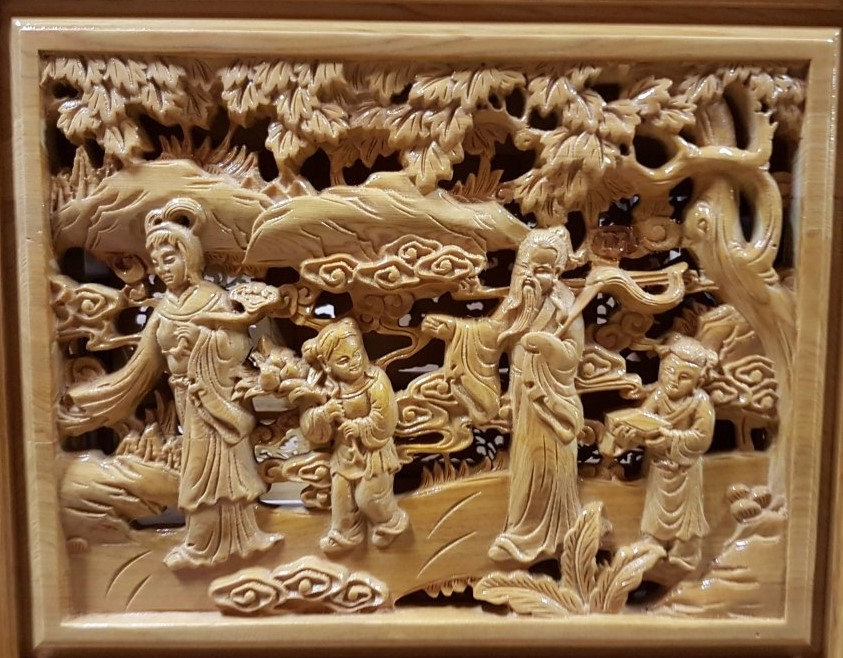
\includegraphics[width=\textwidth]{images/huadu1.jpg}
     \end{subfigure}
     \hfill
     \begin{subfigure}[b]{0.45\textwidth}
         \centering
         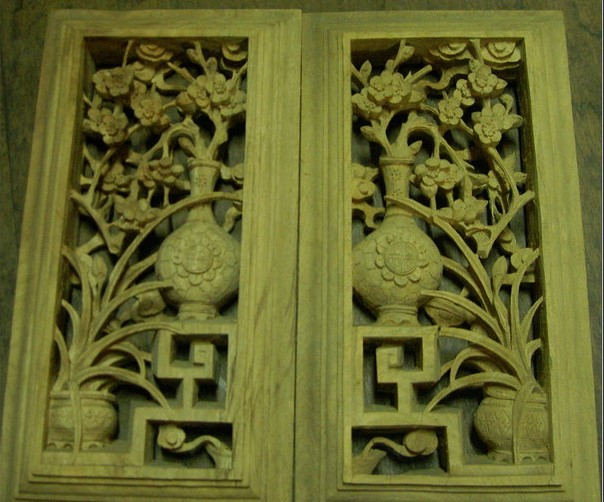
\includegraphics[width=\textwidth]{images/huadu2.jpg}
     \end{subfigure}  
\end{figure}
}:一种雕刻工艺品。
}那大主山所分之脉,\ji{两见大主山,稻香村又云怀中,不写主山,而主山处处映带连络不断可知矣。
}皆穿墙而过。
\ji{好想。
}\par
贾政道:“此处这所房子,无味的很。
”\ji{先故顿此一笔,使后文愈觉生色,未扬先抑之法。
盖钗、颦对峙有甚难写者。
}因而步入门时,忽迎面突出插天的大玲珑山石来,四面群绕各式石块,竟把里面所有房屋悉皆遮住,而且一株花木也无。
\ji{更奇妙!}只见许多异草:或有牵藤的,或有引蔓的,或垂山巅,或穿石隙,甚至垂檐绕柱,萦砌盘阶,\ji{更妙!}
或如翠带飘摇,或如金绳盘屈,或实若丹砂,\zhu{实:果实。
}或花如金桂,味芬气馥,非花香之可比。
\ji{前三处皆还在人意之中,此一处则今古书中未见之工程也。
连用几“或”字,是从昌黎《南山诗》中学得。
\zhu{
昌黎:唐代文学家韩愈,字退之,自谓郡望昌黎,世称韩昌黎。
南山诗:为韩愈的一首五言长诗,诗中连用了 51 个“或”字形容京城长安南边的群山。
}
}贾政不禁道:“有趣!\ji{前有“无味”二字,及云“有趣”二字,更觉生色,更觉重大。
}只是不大认识。
”有的说:“是薜荔藤萝。
\zhu{薜[bì]荔:常绿蔓茎灌木。}
”贾政道:“薜荔藤萝不得如此异香。
”宝玉道:“果然不是。
这些之中也有藤萝薜荔,那香的是杜若蘅芜,
\zhu{
杜若:多年生草本,茎不分枝,根状茎长而横走。
蘅芜[héng][wú]:香草名。
}
那一种大约是茝兰,
\zhu{茝[chǎi]:古书上说的一种香草。}
这一种大约是清葛,
\zhu{葛[gé]:多年生藤本植物,茎蔓生。清:味清香。}
那一种是金䔲草,
\zhu{金䔲[dēng]草:草名。《拾遗记》:“武帝为抚军时,砌下生草三株,状若金。”其状已不可考。}
这一种是玉蕗藤,
\zhu{蕗[lù]:甘草的别名。玉蕗藤:似即甘草,此加玉字,意在状其美,又求与金䔲草对仗,恐并非实有其名。}
红的自然是紫芸,
\zhu{芸[yún]:香草名,即芸香。}
绿的定是青芷。
\zhu{芷[zhǐ]:香草名,即白芷。}
\ji{金䔲草,见《字汇》。
玉蕗,见《楚辞》“菎蕗杂于黀蒸”。
茝、葛、芸、芷,皆不必注,见者太多。
此书中异物太多,有人生之未闻未见者,然实系所有之物,或名差理同者亦有之。
}想来《离骚》《文选》等书上所有的那些异草,\zhu{《离骚》:战国时代楚国诗人屈原的代表作,其中写了许多香草,象征作者所追求的理想和美德。
《文选》:即《昭明文选》,南朝梁昭明太子萧统选编,为现存最早的一部诗文选集。
}也有叫作什么藿蒳姜荨\zhu{藿[huò]蒳[nà]姜荨[qián]:皆为香草名。}\foot{《文选·左思〈吴都赋〉》“姜荨”作“姜彙”。
但本书引用古籍多有改动者,此处作“姜荨”亦通,故不校改。
}的,也有叫什么纶组紫绛的,\zhu{纶[lún]组紫绛:海草名。}还有石帆、水松、扶留等样,
\zhu{
石帆:动物名,珊瑚虫类,暗褐色,形如团扇,故又称“海团扇”。古人以为植物。
水松:植物名。藻类,附生海岸岩石上。
扶留:香草名。
}
\ji{左太冲《吴都赋》。
\zhu{左思《吴都赋》:“石帆水松,东风扶留。”}
}又有叫什么绿荑的,
\zhu{绿荑:木名。亦称“辛夷”、“木笔”,即木兰。}
还有什么丹椒、蘼芜、风连。
\zhu{
丹椒:植物名,即今所谓花椒。
蘼[mí]芜[wú]:香草名。
风连:药草名。
}
\ji{以上《蜀都赋》。
\zhu{左思《蜀都赋》:“或丰绿荑,或蕃丹椒。麋芜布濩于中阿,风连莚蔓于兰皋。”}
}如今年深岁改,人不能识,故皆像形夺名,渐渐的唤差了,也是有的。
”\ji{自实注一笔,妙!}\ping{宝玉已知父亲不是真生气,而是对自己的才学很满意,故敢于在此卖弄学问。
}未及说完,贾政喝道:“谁问你来!”\ji{又一样止法。
}唬的宝玉倒退,不敢再说。
\par
贾政因见两边俱是超手游廊,\zhu{超手游廊:即抄手游廊,院门内两侧环抱的走廊。
}便顺着游廊步入。
只见上面五间清厦连着卷棚,\zhu{五间清厦连着卷棚:“卷棚”是建筑术语,指一种没有正脊的屋面做法,即屋面两坡的连接处不用正脊压盖,而呈一个弧形的转折。
这里“连着卷棚”疑为“连搭卷棚”。
“连搭”正名作“钩连搭”,也是建筑术语,指两个或两个以上的卷棚屋面连接在一起。
“五间清厦连着卷棚”可解为五开间的两卷钩连搭屋面的建筑形式。
}四面出廊,\zhu{四面出廊\foot{
\footPic{四面出廊建筑(图中为紫禁城中和殿)}{simianchulang.jpg}{0.6}
}:四方建筑物的前后左右四个面都有修建在建筑物之外的廊,看起来建筑物是被廊所包围一圈的。
}绿窗油壁,
\zhu{油:油漆。}
更比前几处清雅不同。
贾政叹道:“此轩中煮茶操琴,亦不必再焚名香矣。
\ji{前二处,一曰“月下读书”,一曰“勾引起归农之意”,此则“操琴煮茶”,断语皆妙。
}此造已出意外,诸公必有佳作新题以颜其额,\zhu{以颜其额:在匾额上题字。
颜:这里用作动词,即题字其上。
额:匾。
}方不负此。
”众人笑道:“再莫若‘兰风蕙露’贴切了。
”贾政道:“也只好用这四字。
其联若何?”一人道:“我倒想了一对,大家批削改正。
\zhu{批削:批评改正。}
”念道是:\par
\hop
麝兰芳霭斜阳院,\zhu{麝:麝香为雄麝(一种鹿)之麝香腺中分泌物,干燥后成红棕至暗棕色颗粒。
这里引申为香气。
麝兰:香气馥郁的一种兰。
芳:花草发出的香味。
霭:云雾。
芳霭:和“香飘”对仗,这里是形容香味像云雾一样弥漫飘荡。
}\par
杜若香飘明月洲。
\par
\hop
众人道:“妙则妙矣,只是‘斜阳’二字不妥。
”那人道:“古人诗云:‘蘼芜满手泣斜晖’。
\zhu{
唐代鱼玄机《闺怨》:“靡芜盈手泣斜晖,闻道邻家夫婿归。”
意思是:采了满手的蘼芜,独自在斜晖中哭泣,听说邻居家女子的丈夫已经归来。
}
”众人道:“颓丧,颓丧。
”又一人道:“我也有一联,诸公评阅评阅。
”因念道:\par
\hop
三径香风飘玉蕙,\par
一庭明月照金兰。
\ji{此二联皆不过为钓宝玉之饵,不必认真批评。
}\par
\zhu{三径:汉代蒋诩(音“许”)隐居,荆棘塞门,于舍中竹下开三径,只与求仲、羊仲二人交往。
后常以“三径”泛指庭园间小路。
陶渊明《归去来辞》:「三径就荒,松菊犹存。」
}\par
\hop
贾政拈髯沉吟,意欲也题一联。
忽抬头见宝玉在旁不敢则声,因喝道:“怎么你应说话时又不说了?还要等人请教你不成!”宝玉听说,便回道:“此处并没有什么‘兰麝’、‘明月’、‘洲渚’之类,若要这样着迹说来,就题二百联也不能完。
”贾政道:“谁按着你的头,叫你必定说这些字样呢?”宝玉道:“如此说,匾上则莫若‘蘅芷清芬’四字。
对联则是:\par
\hop
吟成豆蔻才犹艳,\par
睡足酴醿梦也香。
”\ji{实佳。
}\par
\zhu{豆蔻:多年生草本植物,初夏开花成穗状,初为嫩叶所卷,叶渐展花渐开,俗称其未盛开者为“含胎花”,以喻少女。
杜牧《赠别》诗:“娉娉袅袅十三馀,豆蔻梢头二月初”。
因称女子十三、四岁为“豆蔻年华”。
艳:丰满、光彩。
上句说吟成豆蔻诗后才思还很旺盛。
酴醿:音“图迷”,也作“荼蘼”,初夏开花,朵大色白,清香馥郁。
其枝条软垂,常倚架而生。
下句是荼蘼架下香梦沉酣的意思。
}\par
\hop
贾政笑道:“这是套的‘书成蕉叶文犹绿’,
\zhu{书成蕉叶文犹绿:旧有“书成蕉叶文犹绿,吟到梅花句亦香”之联,未详何出。}
不足为奇。
”众客道:“李太白‘凤凰台’之作,全套‘黄鹤楼’,\zhu{李太白“凤凰台”之作,全套“黄鹤楼”:李白《登金陵凤凰台》一诗,在遣词造句方面套用了崔颢的《黄鹤楼》诗。
《黄鹤楼》曾被誉为唐人七律之冠,但李白诗仍能自出新意,寄托深远,故这里说“套得妙”。
}\geng{这一位篾翁更有意思。
\zhu{篾(音“灭”)片:旧时依附于富贵人家,为主子帮闲凑趣的人叫“篾片”。}
}只要套得妙。
如今细评起来,方才这一联,竟比‘书成蕉叶’尤觉幽娴活泼。
视‘书成’之句,竟似套此而来。
”贾政笑说:“岂有此理!”\par
说着,大家出来。
行不多远,则见崇阁巍峨,层楼高起,面面琳宫合抱,\zhu{琳宫:神仙所居之处,这里是说宫室瑰丽犹如仙境。
}迢迢复道萦纡,\zhu{复道:楼阁之间架空连接的通道。
}青松拂檐,玉栏绕砌,金辉兽面,彩焕螭头。
\zhu{
焕:鲜明,光亮;放射(光芒)。
螭[chī]:古代传说中的无角龙。
螭头:这里指古代建筑中一种螭头形的屋顶装饰。
}贾政道:“这是正殿了。
\ji{想来此殿在园之正中。
按园不是殿方之基,\ping{
这两句话的意思大概是,正殿本应该在大观园的正中,但是实际上位于大观园的西北方位。
}西北一带通贾母卧室后,可知西北一带是多宽出一带来的,诸钗始便于行也。
}只是太富丽了些。
”众人都道:“要如此方是。
虽然贵妃崇节尚俭,天性恶繁悦朴,\geng{写出贾妃身分天性。
}然今日之尊,礼仪如此,不为过也。
”一面说,一面走,只见正面\ji{正面,细。
}现出一座玉石牌坊来,上面龙蟠螭护,\zhu{蟠:音“盘”,盘曲地伏着。
螭:音“吃”,古代传说中的无角龙。
}
玲珑凿就。
贾政道:“此处书以何文?”众人道:“必是‘蓬莱仙境’方妙。
”贾政摇头不语。
宝玉见了这个所在,心中忽有所动,寻思起来,倒像那里曾见过的一般,却一时想不起那年月日的事了。
\ji{仍归于葫芦一梦之太虚玄境。
}贾政又命他作题,宝玉只顾细思前景,全无心于此了。
众人不知其意,只当他受了这半日的折磨,精神耗散,才尽辞穷了;再要考难逼迫,着了急,或生出事来,倒不便。
遂忙都劝贾政:“罢,罢,明日再题罢了。
”贾政心中也怕贾母不放心,\ji{一笔不漏。
}遂冷笑道:“你这畜生,也竟有不能之时了。
也罢,限你一日,明日若再不能,我定不饶。
这是要紧之处,更要好生作来!”\geng{一路顺顺逆逆,已成千邱万壑之景,若不有此一段大江截住,直成一盆景矣。
作者从何落笔着想!}\par
说着,引人出来,再一观望,原来自进门起,所行至此,才游了十之五六。
\ji{总住,妙!伏下后文所补等处。
若都入此回写完,不独太繁,使后文冷落,亦且非《石头记》之笔。
}又值人来回,有雨村处遣人来回话。
\ji{又一紧,故不能终局也。
此处渐渐写雨村亲切,正为后文地步。
伏脉千里,横云断岭法。
}
贾政笑道:“此数处不能游了。
虽如此,到底从那一边出去,纵不能细观,也可稍览。
”说着,引众客行来,至一大桥前,水如晶帘一般奔入。
原来这桥便是通外河之闸,引泉而入者。
\ji{写出水源,要紧之极!近之画家着意于山,若不讲水。
又造园囿者,\zhu{囿:音“又”,畜养禽兽的园地,菜园,果园。
}唯知弄莽憨顽石,壅笨冢,\zhu{壅:音“庸”,阻塞。
冢:山。
}辄谓之景,皆不知水为先着。
此园大概一描,处处未尝离水,盖又未写明水之从来,今终补出,精细之至!}贾政因问:“此闸何名?”宝玉道:“此乃沁芳泉之正源,就名‘沁芳闸’。
”\ji{究竟只一脉,赖人力引导之功,园不易造,景非泛写。
}贾政道:“胡说!偏不用‘沁芳’二字。
”\ji{此以下皆系文终之馀波,收的方不突。
}\par
于是一路行来,或清堂茅舍,或堆石为垣,\zhu{垣:音“元”,矮墙,也泛指墙。
}或编花为牖,\zhu{牖:音“友”,窗户。
}或山下得幽尼佛寺,或林中藏女道丹房,\zhu{丹房:道士炼丹的处所。
}或长廊曲洞,或方厦圆亭,贾政皆不及进去。
\ji{伏下栊翠庵、芦雪广、凸碧山庄、凹晶溪馆、暖香坞等诸处,于后文一段一段补之,方得云龙作雨之势。
}因说半日腿酸,未尝歇息,忽又见前面又露出一所院落来,\geng{问卿此居,比大荒山若何?}贾政笑道:“到此可要进去歇息歇息了。
”说着,一径引人绕着碧桃花,\ji{怡红院如此写来,用无意之笔,却是极精细文字。
}穿过一层竹篱花障编就的月洞门,\zhu{花障:有花草攀附的篱笆。
月洞门:圆月形的门洞。
}\ji{未写其居,先写其境。
}俄见粉墙环护,绿柳周垂。
\ji{与“万竿修竹”遥映。
}贾政与众人进去,一入门,两边都是游廊相接。
院中点衬几块山石,一边种着数本芭蕉;那一边乃是一颗西府海棠,\zhu{西府海棠:海棠名贵品种之一。
}其势若伞,丝垂翠缕,葩吐丹砂。
众人赞道:“好花,好花!从来也见过许多海棠,那里有这样妙的。
”贾政道:“这叫作‘女儿棠’,\ji{妙名。
}乃是外国之种。
俗传系出‘女儿国’中,\geng{出自政老口中,奇特之至!}云彼国此种最盛,亦荒唐不经之说罢了。
”\geng{政老应如此语。
}众人笑道:“然虽不经,如何此名传久了?”宝玉道:“大约骚人咏士,以花之色红晕若施脂,轻弱似扶病,\ji{体贴的切,故形容的妙。
}\geng{十字若海棠有知,必深深谢之。
}大近乎闺阁风度,所以以‘女儿’命名。
想因被世间俗恶听了,他便以野史纂入为证,以俗传俗,以讹传讹,都认真了。
”\ji{不独此花,近之谬传者不少,不能悉道,只借此花数语驳尽。
}众人都摇身赞妙。
\par
\clearpage
一面说话,一面都在廊外抱厦下打就的榻上坐了。
\ji{至阶又至檐,不肯轻易写过。
}\zhu{抱厦:原建筑之前或之后接建出来的小房子\foot{\footPic{抱厦(在建筑之前接建)}{baoxia.jpg}{0.6}}}贾政因问:“想几个什么新鲜字来题此?”一客道:“‘蕉鹤’二字最妙。
”又一个道:“‘崇光泛彩’方妙。
”\zhu{崇光泛彩:苏轼《海棠》诗有“东风渺渺泛崇光”之句,写月光笼罩下的海棠。
这里借此诗意点海棠,但“有棠无蕉”,不能兼顾“蕉棠两植”的景物,故宝玉不满意。
}贾政与众人都道:“好个‘崇光泛彩’!”宝玉也道:“妙极。
”又叹:“只是可惜了。
”众人问:“ 如何可惜?”宝玉道:“此处蕉棠两植,其意暗蓄‘红’‘绿’二字在内。
若只说蕉,则棠无着落;若只说棠,蕉亦无着落。
固有蕉无棠不可,有棠无蕉更不可。
”贾政道:“依你如何?”宝玉道:“依我,题‘红香绿玉’四字,方两全其妙。
”贾政摇头道:“不好,不好!”\par
说着,引人进入房内。
只见这几间房内收拾的与别处不同,\geng{特为青埂峰下凄凉与别处不同耳。
}竟分不出间隔来的,\ji{新奇希见之式。
}原来四面皆是雕空玲珑木板,或“流云百蝠”,\zhu{流云百蝠:云朵、蝙蝠组成的图案,“蝠”与“福”谐音,取吉祥多福之意。
}或“岁寒三友”,\zhu{岁寒三友:松、竹经冬不凋,梅则斗寒开花,故有“岁寒三友”之称。
}或山水人物,或翎毛花卉,
\zhu{翎毛[língmáo]:羽毛;国画的一种,以鸟类为主要题材,也说翎毛画。}
或集锦,\zhu{集锦:这里指集合了各种花样的图案。
}或博古,\zhu{博古:这里指以古器物的图形装饰成的工艺品。
}\ji{花样周全之极!然必用下文者,正是作者无聊,撰出新异笔墨,使观者眼目一新。
所谓集小说之大成,游戏笔墨,雕虫之技,无所不备,可谓善戏者矣。
又供诸人同同一戏,妙极!}或万福万寿,\zhu{万福万寿:“万”、“福”、“寿”三个字在庚辰本的书写见页脚注释\foot{\footPic{庚辰本中的“万”}{wan.png}{0.07}\footPic{庚辰本中的“福”}{fu.png}{0.07}\footPic{庚辰本中的“寿”}{shou.png}{0.07}}。
卍:音“万”,梵字,义同“万”,为印度的一种吉祥标相。
}
\ji{前金、玉篆文是可考正篆,今则从俗花样,真是醒睡魔。
\zhu{睡魔:比喻强烈的睡意。在这里的意思大概是耳目一新、生动有趣。}
其中诗词雅谜以及各种风俗字文,一概不必究,只据此等处便是一绝。
}各种花样,皆是名手雕镂,五彩销金嵌宝的。
\zhu{销:熔化金属。}
\ji{至此方见一朱彩之处,亦必如此式方可。
可笑近之园庭,行动便以粉油从事。
}一槅一槅,\zhu{槅:音“格”,物架的分层。
}或有贮书处,或有设鼎处,或安置笔砚处,或供花设瓶、安放盆景处,其槅各式各样,或天圆地方,或葵花蕉叶,或连环半璧。
真是花团锦簇,剔透玲珑。
倏尔五色纱糊就,竟系小窗;倏尔彩绫轻覆,竟系幽户。
\zhu{户:门。}
\ji{精工之极!}且满墙满壁,皆系随依古董玩器之形抠成的槽子。
诸如琴、剑、悬瓶、\ji{悬于壁上之瓶也。
}桌屏之类,虽悬于壁,却都是与壁相平的。
\ji{皆系人意想不到,目所未见之文,若云拟编虚想出来,焉能如此?一段极清极细,后文鸳鸯瓶、紫玛瑙碟、西洋酒令、自行船等文,不必细表。
}众人都赞:“好精致想头!难为怎么想来?”\ji{谁不如此赞?}\par
原来贾政等走了进来,未进两层,便都迷了旧路,左瞧也有门可通,右瞧又有窗暂隔,及到了跟前,又被一架书挡住。
回头再走,又有窗纱明透,门径可行;及至门前,忽见迎面也进来了一群人,都与自己形相一样,——却是一架玻璃大镜相照。
\ping{第四十一回刘姥姥醉酒误入宝玉怡红院,由于没见过大镜子,故错把镜中的自己当作亲家母。}
及转过镜去,\geng{石兄迷否?}一发见门子多了。
\geng{所谓“\sout{投投}[头头]是道”是也。
}贾珍笑道:“老爷随我来。
从这门出去,便是后院,从后院出去,倒比先近了。
”说着,又转了两层纱厨锦槅,\zhu{
纱厨:即碧纱橱,装在房内起隔开作用的一扇一扇的木板墙,也称“隔扇”、“槅扇”。中间两扇平日可以开关,或加挂帘子帷帐,又叫“纱橱”、“纱厨”。
槅心部分常糊以绿纱,故称碧纱橱。
槅:音“格”,物架的分层。
锦槅:即集锦槅,又称“多宝塔”、“博古架”,多以贵重木料制成各种形状的槅子,可摆设各种珍奇古物,是我国古代建筑内檐装修隔断的一种。
}果得一门出去,\geng{此方便门也。
}院中满架蔷薇、宝相。
\zhu{宝相:花名,属蔷薇科。
}转过花障,则见清溪前阻。
\ji{又写水。
}众人咤异:“这股水又是从何而来?”贾珍遥指道:“原从那闸起流至那洞口,从东北山坳里引到那村庄里,又开一道岔口,引到西南上,共总流到这里,仍旧合在一处,\geng{于怡红院总一园之水,是书中大立意。
}从那墙下出去。
”众人听了,都道:“神妙之极!”说着,忽见大山阻路。
众人都道:“迷了路了。
”贾珍笑道:“随我来。
”仍在前导引,众人随他,直由山脚边忽一转,便是平坦宽阔大路,\geng{众善归缘,自然有平坦大道。
}豁然大门前见。
\ji{可见前进来是小路径,此云忽一转,便是平坦宽阔之正甬路也,细极!}众人都道:“有趣,有趣,真搜神夺巧之至!”
\zhu{
搜神夺巧:搜:搜索;神:神奇。谓搜来神奇,夺得巧妙。多用以形容园林景致有巧夺天工之妙。
}
于是大家出来。
\geng{以上可当《大观园记》。
}\par
那宝玉一心只记挂着里边,又不见贾政吩咐,少不得跟到书房。
贾政忽想起他来,方喝道:“你还不去?难道还逛不足!\geng{冤哉冤哉!}也不想逛了这半日,老太太必悬挂着。
快进去,疼你也白疼了。
”\ji{如此去法,大家严父风范,无家法者不知。
}宝玉听说,方退了出来。
\par
\qi{总评:好将富贵回头看,总有文章如意难。
零落机缘君记去,黄金万斗大观摊。
\zhu{
这四句评语的意思大概是:
本回详细描绘了大观园的风光景致,反映了昔日的富贵繁华。
只可惜,再好的文笔也无法阻止衰败乃至抄家的命运。
回忆往昔的繁华,越是漂亮的文笔越会增添哀伤。
痛定思痛,感悟到家族败落的原因是把一万斗黄金投入到大观园的建设中来。
映射到现实,就是曹家五次接驾康熙修造行宫导致亏空,并最终因此而被雍正抄家。
}
}
\dai{033}{大观园试才题对额}
\sun{p17-0}{大观园全景}{俯瞰大观园,一派层峦叠翠、葱蔚洇润气象。
掩映其间的亭台楼阁,或轩峻,或清雅,或玲珑,或温煦,铺陈之直,错落之美,令人惊叹。
}
\sun{p17-1}{曲径通幽处}{只见迎门一带翠嶂挡在前面,往前一望,见白石崚嶒,或如鬼怪,或如猛兽,纵横拱立,上面苔藓成斑,藤萝掩映,其中微露羊肠小径,抬头忽见山上有镜面白石一块,正是迎面留题处。
众人随口各执一词,皆有意俗套敷衍,但等宝玉出来拟定。
宝玉道:“尝闻古人有云:‘编新不如述旧,刻古终胜雕今。
’况此处并非主山正景,原无可题之处,不过是探景一进步耳。
莫如直书‘曲径通幽处’这句旧诗在上,倒还大方气派。
”}
\sun{p17-2}{佳木奇花,雕甍绣槛}{进入石洞来,只见佳木茏葱,奇花熌灼,一带清流,从花木深处曲折泻于石隙之下。
再进数步,渐向北边,平坦宽豁,两边飞楼插空,雕甍绣槛,皆隐于山坳树杪之间。
}
\sun{p17-3}{沁芳亭}{俯而视之,则清溪泻雪,石磴穿云,白石为栏,环抱池沿,石桥三港,兽面衔吐。
桥上有亭。
贾政与诸人上了亭子,倚栏坐了。
议到以何题此,一人云“翼然”,贾政欲题“泻玉”,又令宝玉也拟一个来。
宝玉道:“不若‘沁芳’二字新雅。
”贾政又命宝玉再补一副七言对联,宝玉四顾一望,机上心来,念道:“绕堤柳借三篙翠,隔岸花分一脉香。
”}
\sun{p17-4}{有凤来仪(潇湘馆)}{忽抬头看见前面一带粉垣,里面数楹修舍,有千百竿翠竹遮映,只见入门便是曲折游廊,阶下石子漫成甬路。
上面小小两三间房舍,一明两暗,里面都是合着地步打就的床几椅案。
后院有大株梨花兼着芭蕉。
众人胡乱题词,贾政又命宝玉先说出议论后再来题词,宝玉道:“这是第一处行幸之所,必须颂圣方可。
莫若‘有凤来仪’四字。
”又题一联云:“宝鼎茶闲烟尚绿,幽窗棋罢指犹凉。
”}
\sun{p17-5}{稻香村}{倏尔青山斜阻,转过山怀中,隐隐露出一带黄泥筑就矮墙,墙头上皆用稻茎掩护。
有几百株杏花,如喷火蒸霞一般。
里面数楹茅屋。
外面却是桑、榆、槿、柘,各色树稚新条,随其曲折,编就两溜青篱。
篱外山坡之下,有一土井,旁有桔槔辘轳之属。
下面分畦列亩,佳蔬菜花,漫然无际。
众人道:“莫若直书‘杏花村’妙极。
”宝玉脱口说:“旧诗云‘柴门临水稻花香’,何不用‘稻香村’更妙?”}
\sun{p17-6}{蓼汀花溆}{转过山坡,穿花度柳,抚石依泉,过了荼蘼架,再入木香棚,越牡丹亭,度芍药圃,入蔷薇院,出芭蕉坞,盘旋曲折。
忽闻水声潺湲,泻出石洞,上则萝薜倒垂,下则落花浮荡。
众人说用“武陵源”、“秦人旧舍”命名。
宝玉道:“莫若‘蓼汀花溆’四字。
”}
\sun{p17-7}{花落水流,桃柳争艳}{大家攀藤抚树过去。
只见水上落花愈多,其水愈清,溶溶荡荡,曲折萦纡。
池边两行垂柳,杂着桃杏,遮天蔽日,真无一些尘土。
}
\sun{p17-8}{蘅芜苑}{忽见柳阴中又露出一个折带朱栏板桥来,度过桥去,诸路可通,便见一所清凉瓦舍,一色水磨砖墙,清瓦花堵。
那大主山所分之脉,皆穿墙而过。
步入门时,忽迎面突出插天的大玲珑山石来,四面群绕各式石块,竟把里面所有房屋悉皆遮住,而且一株花木也无。
只见许多异草。
}
\sun{p17-9}{天仙宝境}{行不多远,则见崇阁巍峨,层楼高起,面面琳宫合抱,迢迢复道萦纡,青松拂檐,玉栏绕砌,金辉兽面,彩焕螭头。
只见正面现出一座玉石牌坊来,上面龙蟠螭护,玲珑凿就。
宝玉见了这个所在,心中忽有所动,寻思起来,倒像那里曾见过的一般,却一时想不起那年月日的事了。
}
\sun{p17-10}{沁芳闸}{一大桥前,水如晶帘一般奔入。
原来这桥便是通外河之闸,引泉而入者。
贾政因问:“此闸何名?”宝玉道:“此乃沁芳泉之正源,就名‘沁芳闸’。
”}
\sun{p17-11}{红香绿玉(怡红院)}{绕着碧桃花,穿过一层竹篱花障编就的月洞门,俄见粉墙环护,绿柳周垂。
贾政与众人进去,一入门,两边都是游廊相接。
院中点衬几块山石,一边种着数本芭蕉;那一边乃是一颗西府海棠,其势若伞,丝垂翠缕,葩吐丹砂。
贾政因问:“想几个什么新鲜字来题此?”宝玉道:“此处蕉棠两植,其意暗蓄‘红’‘绿’二字在内。
若只说蕉,则棠无着落;若只说棠,蕉亦无着落。
固有蕉无棠不可,有棠无蕉更不可。
题‘红香绿玉’四字,方两全其妙。
”}
\sun{p17-12}{怡红院室内}{进入房内,竟分不出间隔来的,原来四面皆是雕空玲珑木板,或“流云百蝠”,或“岁寒三友”,或山水人物,或翎毛花卉,或集锦,或博古,各种花样,皆是名手雕镂,五彩销金嵌宝的。
一槅一槅,或有贮书处,或有设鼎处,或安置笔砚处,或供花设瓶、安放盆景处,其槅各式各样,或天圆地方,或葵花蕉叶,或连环半璧。
真是花团锦簇,剔透玲珑。
倏尔五色纱糊就,竟系小窗;倏尔彩绫轻覆,竟系幽户。
且满墙满壁,皆系随依古董玩器之形抠成的槽子。
诸如琴、剑、悬瓶、桌屏之类,虽悬于壁,却都是与壁相平的。
}
\sun{p17-13}{问得清溪何许来}{院中满架蔷薇、宝相。
转过花障,则见清溪前阻。
众人咤异:“这股水又是从何而来?”贾珍遥指道:“原从那闸起流至那洞口,从东北山坳里引到那村庄里,又开一道岔口,引到西南上,共总流到这里,仍旧合在一处,从那墙下出去。
”众人听了,都道:“神妙之极!”说着,忽见大山阻路。
众人都道:“迷了路了。
”}
\sun{p17-14}{峰回路转见大门}{贾珍笑道:“随我来。
”仍在前导引,众人随他,直由山脚边忽一转,便是平坦宽阔大路,豁然大门前见。
众人都道:“有趣,有趣,真搜神夺巧之至!”于是大家出来。
}


